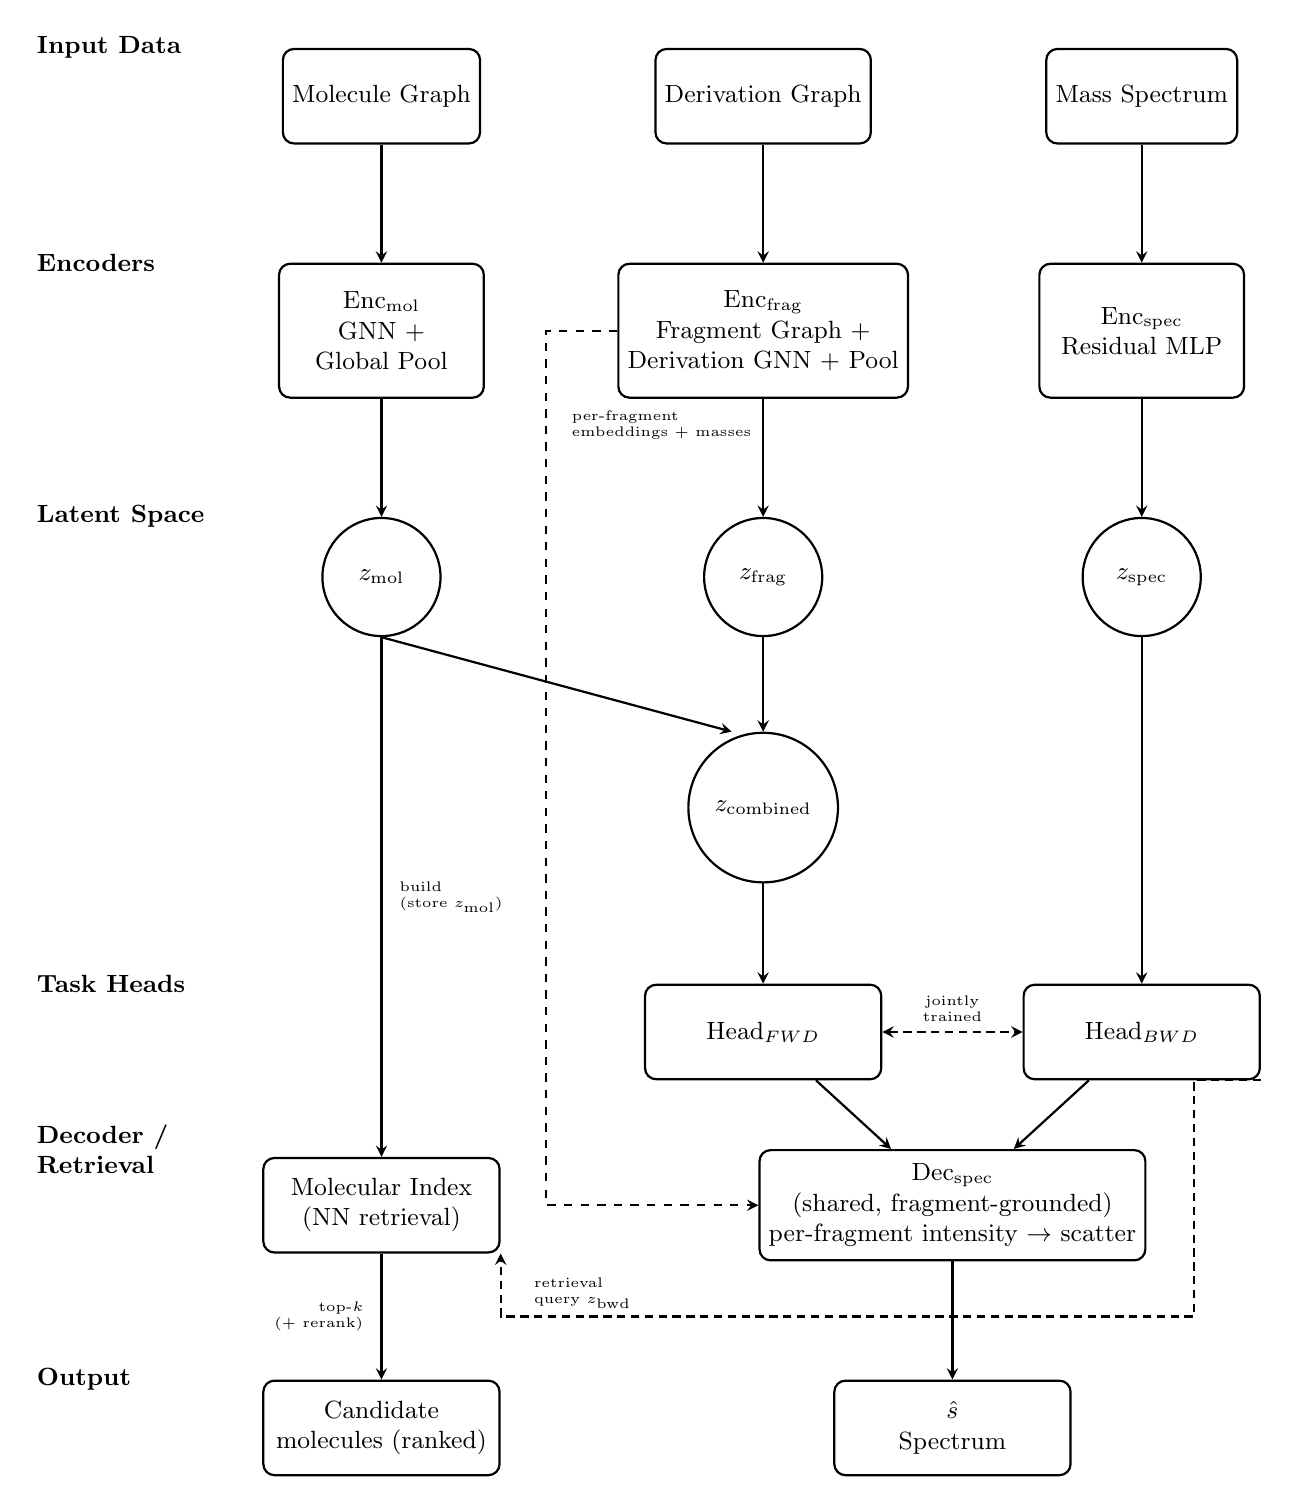
\begin{tikzpicture}[
  node distance = 15mm and 22mm,
  >=stealth,
  inputNode/.style    ={rectangle, rounded corners, draw=black, thick, minimum width=2.2cm, minimum height=1.2cm, text centered, align=center, font=\small},
  encoderNode/.style  ={rectangle, rounded corners, draw=black, thick, minimum width=2.6cm, minimum height=1.7cm, text centered, align=center, font=\small},
  latentNode/.style   ={circle, draw=black, thick, minimum width=1.5cm, text centered, align=center, font=\small},
  headsNode/.style    ={rectangle, rounded corners, draw=black, thick, minimum width=3.0cm, minimum height=1.2cm, text centered, align=center, font=\small},
  decoderNode/.style  ={rectangle, rounded corners, draw=black, thick, minimum width=3.0cm, minimum height=1.4cm, text centered, align=center, font=\small},
  outputNode/.style   ={rectangle, rounded corners, draw=black, thick, minimum width=3.0cm, minimum height=1.2cm, text centered, align=center, font=\small},
  arrow/.style        ={->, thick},
  dashedArrow/.style  ={dashed, ->, thick},
  queryArrow/.style   ={densely dashed, ->, thick},
  syncArrow/.style    ={<->, densely dashed, thick},
  groupLabel/.style   ={font=\bfseries\small, anchor=west}
]
\usetikzlibrary{positioning, calc}

% ---- shift the MAIN pipeline right (tune xshift as you like) ----
\begin{scope}[xshift=18mm]

% Define fixed x-coordinate for all labels
\coordinate (labelX) at (-45mm, 0);

% ================== INPUT ROW ==================
\node[inputNode] (MOL)  {Molecule Graph};
\node[inputNode, right=of MOL] (FRAG) {Derivation Graph};
\node[inputNode, right=of FRAG] (SPEC) {Mass Spectrum};
\node[groupLabel] at (labelX |- MOL.north) {Input Data};

% ================== ENCODER ROW ==================
\node[encoderNode, below=of MOL]  (EncMol) {$\mathrm{Enc}_{\mathrm{mol}}$\\GNN +\\Global Pool};
\node[encoderNode, below=of FRAG] (FragSetEnc) {$\mathrm{Enc}_{\mathrm{frag}}$\\Fragment Graph +\\Derivation GNN + Pool};
\node[encoderNode, below=of SPEC] (EncSpec) {$\mathrm{Enc}_{\mathrm{spec}}$\\Residual MLP};
\node[groupLabel] at (labelX |- EncMol.north) {Encoders};

\draw[arrow] (MOL) -- (EncMol);
\draw[arrow] (FRAG) -- (FragSetEnc);
\draw[arrow] (SPEC) -- (EncSpec);

% ================== LATENT ROW ==================
\node[latentNode, below=of EncMol]     (ZM) {$z_{\mathrm{mol}}$};
\node[latentNode, below=of FragSetEnc] (ZF) {$z_{\mathrm{frag}}$};
\node[latentNode, below=of EncSpec]    (ZS) {$z_{\mathrm{spec}}$};

\node[latentNode, minimum width=1.9cm, below=12mm of ZF] (ZFUSED) {$z_{\mathrm{combined}}$};
\node[groupLabel] at (labelX |- ZM.north) {Latent Space};

\draw[arrow] (EncMol) -- (ZM);
\draw[arrow] (FragSetEnc) -- (ZF);
\draw[arrow] (EncSpec) -- (ZS);

% fan-in (avoid stacking)
\draw[arrow] (ZM.south) -- ($(ZFUSED.north)+(-4mm,0)$);
\draw[arrow] (ZF.south) -- (ZFUSED.north);

% ================== HEADS ROW (LogVars removed) ==================
\node[headsNode, below=44mm of ZF] (HdFwd) {Head$_{FWD}$};
\node[headsNode, below=44mm of ZS]  (HdBwd) {Head$_{BWD}$};
\node[groupLabel] at (labelX |- HdFwd.north) {Task Heads};

\draw[arrow] (ZFUSED) -- (HdFwd);
\draw[arrow] (ZS) -- (HdBwd);
\draw[syncArrow] (HdFwd) -- (HdBwd) node[midway, above, font=\tiny, align=center] {jointly\\trained};

% ================== DECODER ROW (shared, fragment-grounded spectrum decoder) ==================
\node[decoderNode, minimum width=3.6cm] (DecSpec) at ($(HdFwd)!0.5!(HdBwd)+(0,-22mm)$) {$\mathrm{Dec}_{\mathrm{spec}}$\\(shared, fragment-grounded)\\per-fragment intensity $\rightarrow$ scatter};
\node[groupLabel, align=left] at (labelX |- DecSpec.north) {Decoder /\\Retrieval};

% both task heads feed the single shared spectrum decoder as a conditioning latent
\draw[arrow] (HdFwd) -- (DecSpec);
\draw[arrow] (HdBwd) -- (DecSpec);

% the decoder is fragment-grounded: it also consumes the per-fragment embeddings
% and masses from the fragment encoder, so each peak lands at a fragment's own mass
\coordinate (PFx) at ($(FragSetEnc.west)+(-9mm,0)$);   % vertical run of the per-fragment skip
\draw[dashedArrow] (FragSetEnc.west) -- (PFx) |- (DecSpec.west);
\node[font=\tiny, align=left, anchor=west] at ($(PFx)+(2mm,-12mm)$)
  {per-fragment\\embeddings + masses};

% ================== OUTPUT ROW ==================
\node[outputNode, below=of DecSpec] (SPEC_HAT) {$\hat{s}$\\Spectrum};

\draw[arrow] (DecSpec) -- (SPEC_HAT);

\end{scope} % end pipeline shift

% ================== RETRIEVAL (INDEX) + OUTPUT (CANDIDATES), MOL COLUMN ==================
% The molecular index is a retrieval store, not a model output: it holds the gallery of
% z_mol vectors. It sits at the decoder row as the backward-path counterpart of Dec_spec,
% and the actual output of the retrieval path is the ranked candidate list below it.
\node[outputNode, at=(MOL |- DecSpec)]  (INDEX) {Molecular Index\\(NN retrieval)};
\node[outputNode, at=(MOL |- SPEC_HAT)] (CAND)  {Candidate\\molecules (ranked)};
\node[groupLabel] at (labelX |- CAND.north) {Output};

% build: every gallery molecule's latent z_mol is stored in the index
\draw[arrow] (ZM.south) -- (INDEX.north)
  node[pos=0.5, right=1mm, font=\tiny, align=left] {build\\(store $z_{\mathrm{mol}}$)};
% the retrieval step returns a ranked candidate list (top-k, optionally re-ranked)
\draw[arrow] (INDEX.south) -- (CAND.north)
  node[pos=0.5, left=1mm, font=\tiny, align=right] {top-$k$\\(+ rerank)};

% retrieval query (inference): the backward-head latent z_bwd is the nearest-neighbour
% query against the stored z_mol vectors. Routed under the decoder so it only crosses
% the decoder->spectrum arrow, then up into the index's south-east corner.
\coordinate (Qrx)  at ($(DecSpec.east)+(6mm,0)$);            % lane just right of the decoder
\coordinate (Qund) at ($(DecSpec.south)+(0,-7mm)$);          % lane just below the decoder
\coordinate (Qa)   at (Qrx |- HdBwd.south);
\coordinate (Qb)   at (Qrx |- Qund);
\coordinate (Qc)   at (INDEX.south east |- Qund);
\draw[queryArrow]
  (HdBwd.south east) -- (Qa) -- (Qb) -- (Qc) -- (INDEX.south east);
\node[font=\tiny, align=left, anchor=west] at ($(INDEX.south east)+(3mm,-5mm)$)
  {retrieval\\query $z_{\mathrm{bwd}}$};

% Loss terms are intentionally omitted from this architecture overview; the full
% training objective is given in the loss table / losses section of the text.

\end{tikzpicture}
